\documentclass[conference]{IEEEtran}
%\usepackage{geometry}                % See geometry.pdf to learn the layout options. There are lots.
%\geometry{letterpaper}                   % ... or a4paper or a5paper or ... 
%\geometry{landscape}                % Activate for for rotated page geometry
%\usepackage[parfill]{parskip}    % Activate to begin paragraphs with an empty line rather than an indent
\usepackage{graphicx}
\usepackage{amssymb}
\usepackage{epstopdf}
%\usepackage[margin=1.5in]{fullpage}
\DeclareGraphicsRule{.tif}{png}{.png}{`convert #1 `dirname #1`/`basename #1 .tif`.png}
%\usepackage{}
\usepackage{color}
\definecolor{Orange}{rgb}{1,0.5,0}
\definecolor{HBGreen}{rgb}{0,0.8,0}
\newcommand{\todo}[1]{\textsf{\textbf{\textcolor{Orange}{[Todo: #1]}}}}
% Macro for writing in the margin comments on what is left to be done.
\newif\ifdraft
               \drafttrue
               %\draftfalse
\ifdraft
\newcounter{ournotecounter}
\newcommand{\ournote}[1]{%
\textsf{\textbf{\textcolor{Orang}{[#1]}}}}
\newcommand{\alnote}[1]{%
\textsf{\textbf{\textcolor{HBGreen}{[#1]}}}}
\typeout{Compiling in draft mode.}
\else
\newcommand{\ournote}[1]{}
\newcommand{\bigournote}[1]{}
\typeout{Compiling in final mode.}
\fi

\title{Estimating vehicle carbon dioxide emissions through smartphone sensors}
%\subtitle{Using mobile sensing data}
\author{\IEEEauthorblockN{Anders Lehmann}
\IEEEauthorblockA{Department for Computer Science\\
University of Aarhus\\
Email: anders@hih.au.dk}
\and
\IEEEauthorblockN{Henrik Blunck}
\IEEEauthorblockA{Department for Computer Science\\
University of Aarhus\\
Email: blunck@cs.au.dk}
\and
\IEEEauthorblockN{Niels Olof Bouvin}
\IEEEauthorblockA{Department for Computer Science\\
University of Aarhus\\
Email: bouvin@cs.au.dk}
\and
\IEEEauthorblockN{Allan Gross}
\IEEEauthorblockA{Department of Business Development and Technology\\
University of Aarhus\\
Email: agr@auhe.au.dk}

}
\date{October 2015}                                           % Activate to display a given date or no date

\begin{document}
\maketitle
\begin{abstract}
Carbon dioxide emissions from transport constitutes a large, and growing, part of the total carbon emissions. We present a model to estimate carbon dioxide emissions from passenger cars on basis of GPSby using GPS data and accelerometer datae gathered from the driver's or passengers' smartphone apps. The model will enable a more detailed emission inventory, both in terms of location and time.\todo{how are location and especially time to be understood here?}
 \todo{move to end:?} As part of an experiment to establish ground truth, a method for measuring fuel consumption without instrumenting vehicles is presented. 
 As part of this estimation model,  aA method for discerning between different driving modes is presented, using the K-means clustering method. This method will increase the accuracy of the emission model by estimation of increased fuel consumption while accelerating and decreased fuel consumption while braking, as well as estimate idle time.

\end{abstract}
\pagenumbering{arabic}	
\todo{fix figures, legends labels, axis}

\todo{niels kommentarer}
\todo{Henriks kommentarer}
\todo{conclusion futurework acceleration}
\todo {models mention kmeans}
\todo{results more in kmeans, relation to emissions}
\todo{results comparison to other methods, hhmm, measurement of accurcy, relation to emissions}


\section{Introduction}

The proliferation of smartphones brings new opportunities to researchers who are studying the behaviour of modern human beings. For research in mobility and transport the proliferation of smartphones yields the potential to lower the cost for gathering relevant data to near zero \cite{Liu2013}.
In this project, smartphones are a central requisite as an tool information and data gathering tool. The main idea in the project is to gather from real life activities, create models to interpret the data, and visualisations from the output of the models. 

In modern societies, carbon emissions from transport are a large and growing part of the total carbon emissions from human activities. For instance, in Denmark the emission of carbon dioxide from transport was 24 \% of the total Carbon emissions in 2012 \cite{nielsen2014}, and road transport is responsible for 67 \% of the Carbon emissions from transport. In order to be able to create viable measures to lower the carbon emissions from passenger transport, there is a need for more detailed models quantifying these emissions. By using data from smartphones we aim to obtain more accurate information on where and when emissions from transport are created. These models can help policy makers and planners make informed decisions on future changes to the road transport system and related infrastructure.

As Carbon emissions are closely related to the fuel consumption, experiments were designed and carried out which gathered from an onboard smartphone  driving-related data and data on the amount of fuel consumed.

\todo{can be ommited?:}
To accurately model Carbon emissions from smartphone data, an experiment was performed in order to establish a ground truth\todo{ground truth: explain what and why?}. 

We chose to use some old car \todo{exact details? btw, use different cars for a broader range of experiments?} for the experiments and thus 
\todo{this sounds like a poor choice and excuse? Can we say that we aim for getting data also from all includung old cars? Btw, what about the instrumenting software that you had trouble with but which our developers now have instrumented on our department car? Would that make that your statement above obsolete?} had to create an accurate fuel consumption measuring method, which did not involve instrumenting the vehicles. 


The remained of the paper is organized as follows:
In Section \ref{sec:relwork} we review related work, including methods for measuring the fuel consumption and for creating related models of fuel consumption from sensor data  Additinoally, we briefly review methods to determine different driving styles and driving modes.
In Section \ref{sec:modeling} the models used to convert the experimental data into emission data are presented. 
The results of the experiments which partly relate to fuel consumption measurement and modeling and partly to reliable detection of driving modes, are presented in Section \ref{sec:results} and the paper is concluded in Section \label{sec:conclusions}.
\section{Related work}
\label{sec:relwork}
 Carbon emissions from passenger cars are closely linked to fuel consumption, as the primary source of carbon dioxide is the combustion of hydrocarbons. To model the fuel consumption from  data from smartphones, we need to establish a correlation between the observed data, and the consumed fuel. We provide an overview of existing methods for modelling fuel consumption via instrumenting vehicles or modelling best on standardised driving cycles.

In \cite{hilpert201} the authors propose a real time data gathering system and model based on On Board Diagnostics system (OBD2). From the data gathered, emissions from the vehicle and a product carbon footprint are calculated, by a simple relation between airflow into the engine, the stoichiometric fuel to air ratio, and the carbon dioxide emission factor for gasoline/diesel. No actual data are reported. For the old car we used in the experiment, the OBD2 option was not available. 

For detection and analysing of driving styles for prevention of car crashes, the authors in \cite{Johnson2011} make use of sensor fusion of sensors from smartphones, and data obtained from the internal CAN \footnote{"controller area network", an intra vehicle network standard ISO 11898} bus in cars. The authors show that it is possible to accurately detect driving events and to classify the aggressiveness of the driver from the used sensor. We want to be able to determine turns as well as the agresiveness of accelerating and braking event.

Models for the emission from gasoline cars are evaluated in \cite{Silva2006}, by combining simulation with measurements done with a combination of data from the OBD2 \footnote{OnBoard Diagnostic 2, a standard for communication between vehicle test equipment and vehicle}, and sensors placed in the tail pipe. Three different numerical models were compared to the measurements. The same instrument setup (OBD2 and tailpipe sensors were used in \cite{Frey}, where the goal was to estimate emission factors for different driving modes. One conclusion is that the emission pattern for cold start driving is significantly different from steady state driving. As our experiment is designed to be able to model the most used driven patterns, we have focused on warm engine mode of operation, thus we perform a warm up drive before the actual test run.

The paper \cite{Lee2010} provides an overview of different projects using mobile sensing platforms. The paper is mostly concerned with network topologies for mobile sensor network and backend support for data storage and retrieval, but also has some input on different sensors used.

In \cite{Boriboon} the effects of the road grade (road inclination) on fuel consumption is investigated, through the use of OBD2 measurements and models. Two different routes between a Origin-Destination pair (one route through a flat area, and one through a mountain pass) are compared in multiple trips. The fuel consumption is determined from a binary fuel cut signal from the OBD2 data, and compared to fuel consumption modelled by CMEM (comprehensive modal emission model). We have chosen to focus on a flat course, in order not to have the road grade as a consideration. We have also chosen to use a single course with the same point as start and finish, as our test course.

For using accelerometers to determine transportation modes \cite{Hemminki2013} gives an overview of methods, applications and problems. Examples of how to use Hidden Markov Models classifiers to discern between different transportation modes are given. \cite{mun_peir_2009} adds a personalized environmental impact report generated from mobile sensed data. Where these papers focus on transportation modes, ie. which kind of transportation, we focus on how the driving is performed.

The authors in \cite{markus2014} give an example of discerning electric vehicles from combustion engine vehicles, by using accelerometer data to measure the revolutions of combustion engine in idle mode. In idle mode electric vehicles do not have a turning engine. The paper shows how signal analysis combined with classifiers can detect vehicle differences from engine vibrations. The paper also shows that noise when cars are driving makes engine detection hard.

To monitor road condition the authors of \cite{ghose2012road} proposes to use the accelerometer to measure road quality and if pot holes are detected to alert at what position the pot hole is located.

Development and yearly reporting of national emission inventories was agreed on in the terms of the Kyoto protocol. This has led to the development of rigorous models and protocols for reporting the total national emission. To be able to make detailed reports of the transportation related emissions the COPERT \footnote{http://emisia.com/copert} \cite{Mellios2011} program was developed as a European transport emission model.

To test the long-term impact of Eco-driver training the authors of \cite{beusen2009using} used GPS and OBD2 to get information on engine RPM and other engine parameters. This information was used to model some driving modes,as accelerating, braking and at which RPM gear shifts were performed.

In the mentioned papers a cross section of methods and tools for estimation of fuel consumption and emission from light duty vehicles and passenger cars is presented. The tools used in the papers are OBD2, GPS and tail pipe emission sensors. The methods used are controlled driving cycles, simulation models, classifiers and sensor fusion.

There is also a host of commercial and free apps offering driving style analysis directly on your smartphone. An example is goDriveGreen\footnote{https://itunes.apple.com/us/app/godrivegreen/id411510594}
 
The work in this paper extends and complements the work in the above mentioned papers, by using measurements from smartphone accelerometers and by controlled measurement of fuel consumption, and by exploring a different classifier than presented in the above papers. This work can be used for vehicles that do not have an OBD2 connector and cannot be instrumented with mass flow meters for measuring fuel consumption as in \cite{haan2000,Honicky}


%\input{mobilesensing}
%\input{emission_models}
%\input{hypoteser}
\section{Experiment}
An accurate model for Carbon emission from transport, can be derived from an accurate model of fuel consumption of vehicles, since the Carbon emissions are related to the combustion of fuel. 
To get a baseline for the fuel consumtption model, an experiment was performed. Data from a smartphone was combined with accurate measurements of fuel consumption. 

Researchers have reported fuel consumption measurements by instrumenting the vehicles with flow gauges in the fuel line. These measurements allow for realtime measurements of the fuel consumption. For this experiment flow meters were not available, nor was it possible to instrument the cars. Instead an elaborate measurement procedure was developed to attain accurate fuel consumption measurements.

\subsection{Route selection}
To select a route for the experiment, a number of criteria was considered. The length of the route should be long enough to have a measurable consumption, but short enough to be repeatable, and certainly less than the range of a tankful of fuel. The route should comprise different driving patterns (urban, rural, high speed/low speed) to simulate real life driving patterns. 

The route was chosen to mainly be in an urban traffic setting. The urban setting was chosen in order to get as many accelerations and idle periods a possible. The route did contain a short distance on a rural highway in order to have high speed measurements as well.

The length of the route was chosen to be 13 km, which was short enough to be repeated, and long enough to make measurement of fuel consumption possible. The fuel consumption for the route was approximately one liter of fuel, depending on driving style.

To prevent cold start effects to affect the tests, the vehicle is driven until the engine has reached the operating temperature before starting the test. The chosen course was run a number of times and the fuel consumption was determined after each run.

\subsection{Measurement of fuel consumption}

As it was not possible to install mass flow meters in the test vehicles the following procedure was developed to determine the fuel consumption. A the start of the course the gas tank was filled and  the fuel level in the gas tank funnel was measured. After the course was completed, gas was refilled so the same level of gas in the funnel, from a fuel canister. The weight of the fuel canister was measured before and after the gas filling process, to determine the amount of fuel refilled, and thus the consumption of fuel for the trip. To get a reproducible reading of the weight of the canister the weight has to be placed at the same place, with the same orientation, for each measurement. An ordinary kitchen scale with 1g accuracy was used in the experiment. In order to reduce the effect of wind on the measurement the scale and canister was placed in a cardboard box during the measurement.

This elaborate method was needed since the use of gas dispenser at the gas station, proved inaccurate. The main problem of using the fuel dispenser to measure the amount of fuel consumed driving the test route, is that it is hard to get the same filling level at each each filling. Using the automatic filling stop mechanism is unreliable, as the filling level becomes dependant on how much foam the filling process has created in the tank and the funnel. This creates large deviations of the amount of fuel to replenish the gas after the test runs. 

By accurately measure the filling level and refill the gas from a canister, made it possible to have very small differences between subsequent runs, with equal driving styles. 

The accuracy of the measurement can be estimated by inspecting the uncertainty of the individual steps of the measurement. The tank filling level can be measured with an accuracy of less than one cm, and since the diameter of the funnel is five cm the maximum error of the fuel measurement will be less than 20 cm\textsuperscript{3} or 20 ml, which is 2 \% if the total fuel refill is one liter.

\section{Modelling emissions}

To model the carbon emissions from single vehicle trips, the fuel consumption is modelled from data obtained from an onboard smartphone.

The data received from smartphones comes from a variety of sensors. For this experiment we used the accelerometer and GPS sensors. From the GPS sensor information on speed, heading and location is obtained, and from the accelerometer the size and direction of acceleration is gathered.

\subsection{Method from National Emission model}

In the COPERT IV emission modelling program, emission from warm combustion engines is modelled from the speed of the vehicle. As an example the emission $CO_2$ is modelled by modelling the fuel consumption of the vehicle, since the $CO_2$ emission is directly linked to the amount of fuel burned in the engine. Equation \ref{emission} is an example of how COPERT IV models the fuel consumption of a petrol driven passenger car as a function of the speed of the vehicle \cite{Ntziachristos2012}. There is a similar equation covering the fuel consumption of diesel cars. The constants $a-e$ are found by testing and differs by car type, engine size, year of manufacturing, and regulation. The COPERT IV program uses mean values for all tested vehicles within a particular class of vehicles.

\begin{equation}
	FC_{warm} = \frac{a + c*v + e*v^2}{1 + b*v + d*v^2}
	\label{emission}
\end{equation}

Figure \ref{FC} shows an example of the fuel consumption of passenger cars from 1999 versus speed. The consumption is measured in $l/km$, and is seen to have a minimum at app. $80 km/h$ for petrol cars and app. $60 km/h$ for diesel driven cars. The fuel consumption is high for low speeds due to the fact that the engine is underused, and the fuel consumption is high at high speeds due to increased wind forces on the vehicle. The equation is only defined for the speed range $10 - 130 km/t$
 
\begin{figure}[h]
  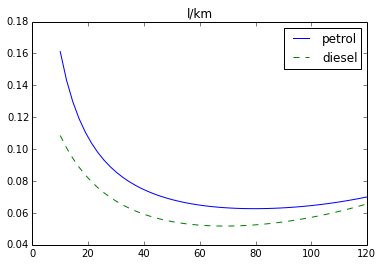
\includegraphics[scale=0.5]{fc_dieselpetrol}
  \caption{Fuel consumption versus speed for 1999 passenger car.}
  \label{FC}
\end{figure}

From fuel consumption the carbon dioxide emission can be modelled under the assumption of perfect combustion. If all carbon atoms in the fuel is oxidised into carbon dioxide, we only need to know how many carbon atoms there are in a liter of fuel.

\subsection{Single trip emission model}
The model developed in this paper builds upon the work from the national emission inventories. By using the instantaneous speed data obtained from Smartphones, and the fuel consumption versus speed curve from the COPERT program, instantaneous emissions can be calculated.

By assuming a constant speed between two measurements of the speed of the vehicle, and by measuring the distance between the two speed measurements, we calculate the fuel consumption for the distance by multiplying the distance with the fuel consumption given by equation \ref{emission}. The fuel consumption, and thus the carbon dioxide emission, for a single trip can then be calculated as the sum of the instantaneous consumptions.

One problem with the above method is that the fuel consumption model, defined in equation \ref{emission} is only valid for speeds between $10$ and $130 km/t$. This means that fuel consumption when the vehicle is idle (for instance waiting for green light at an intersection), is probably modelled too high.


\subsection{Emission model for accelerating vehicles}

To model the emission from accelerating vehicles, we first need to establish the different forms of driving modes. For each driving mode a emission model have to be employed.

In order to model the effect of vehicle acceleration, we divide the trip into six driving patterns, idle, forward acceleration, deceleration, cruise at constant speed, left turn and right turn. Reversing is not considered in this project, partly because we have no data and partly because it is an infrequent driving pattern. 

Gravity 

Position of smartphone

To detect acceleration


Turning

Cruise is characterised by
 For cruising the emission model from equation \ref{emission}, can be used, since the speed is constant.

Idle

The emission model for the braking and idle driving mode, can be the same, since regenerative braking is not used in many passenger cars with only a combustion engine.

K-means



 
\section{Results}

The experiment was carried out in Holstebro, Denmark with a diesel Citr\"oen Xantia car. The data collection was done with an iPhone 4s running an app called SensorLog\footnote{http://sensorlog.berndthomas.net/}. The data gathered consisted of GPS, accelerometer. The GPS is sampled at approximately 90 hz.

A total of 22 test runs were driven, three test was not completed due to driver errors, leaving
usable data from 19 test runs. In the processing of data it became apparent that the original way of measuring fuel consumption, by using the meter at the gas pump, and thus were the more reliable measurement method developed (as seen in figure \ref{measured}). Only two test runs were completed with the new method.

\begin{table}
\begin{tabular}{| l | r |}
\hline 
number of trips & 19 \\[0.1cm] \hline
number of datapoints & $12*10^6$\\[0.1cm] \hline
height difference & 6 m\\[0.1cm]
\hline 

\end{tabular}
\label{datatable}
\caption{Description of input data}
\end{table}
map of trip

\begin{figure}[h]
	\centering
	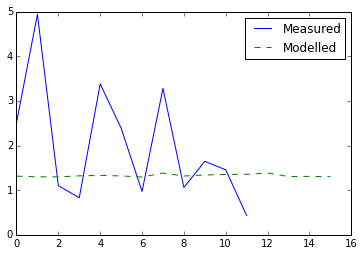
\includegraphics[width=0.45\textwidth]{Measured_consumption}
  \caption{The measurement using the pump meter is quite unreliable}
  \label{measured}
\end{figure}

The modelled fuel consumption uses the equation \ref{emission} for each sample point. The speed is the speed estimate gained from the GPS data. Each consumption factor derived from  equation \ref{emission} is the multiplied with the distance from the previous sample point. The distance is calculated from the GPS location and the previous GPS location, using the haversine formula \cite{rick1999deriving} to take the spherical nature of the earth into account.

The modelled fuel consumption from the test has a mean value of 1.32 liters, and a standard deviation of 0.03.

An example speed curve of a run can be seen in figure \ref{speed}.

\begin{figure}[h]
	\centering
	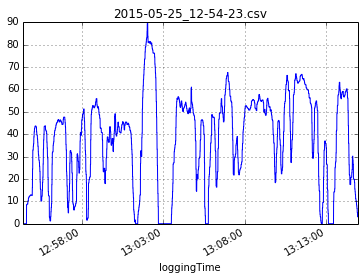
\includegraphics[width=0.45\textwidth]{speed}
  \caption{A speed trace for a test run}
  \label{speed}
\end{figure}

The different driving patterns are apparent in the figure, as the large number of speed changes suggests.

\subsection{Acceleration data}

The data from the accelerometer of the smartphone, is used for determine the driving patttern of the driver. Part of the driving pattern is determined by road conditions, such as intersection, stoplights, curves and turning. Other patterns are due to personal driving style, ie. heavy acceleration, overtaking and braking versus more smooth driving, and lastly some patterns are due to traffic conditions, like congested, accidents and slow or fast moving vehicles.
\begin{figure}[h]
	\centering
	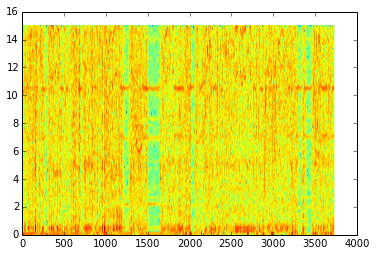
\includegraphics[width=0.45\textwidth]
{specgram}
  \caption{A spectogram of the magnitude of the acceleration}
  \label{spectogram}
\end{figure}
In figure \ref{spectogram} the magnitude of the acceleration is shown in a spectogram. The x-axis is time (sample number), and the y-axis is the frequency spectrum of the acceleration signal. Form the figure it can be seen that the idle running of the motor, when standing still is very visible, while the motor frequency is not discernible while the vehicle is moving, due to vibrations from the wheels moving on the road.

The spectrogram indicates that the accelerometer signal can be used for detecting an idle running engine in a stationary vehicle.

To be able to discern different driving patterns a simple K-means clustering algorithm was used. There are six driving odes that are of interest: idle, forward acceleration, braking, cruising, left turn, and right turn, thus the number of clusters was chosen to six. Figure \ref{cluster} shows the results of the K-means clustering algorithm on the data from 19 test runs. The clustering is performed separately on each test run, but since the position and orientation of the smartphone was kept the same in all tests (parallel to the vehicle, with X toward the front face (Z) up), we present the results in the same figure. The upper figure shows the X and Y part of the cluster centers, and the two lower figures shows the X, Z part and Y,Z part respectively. There are many cluster centers close the the origin of the graph, corresponding to either idle or cruising driving mode. Many of the test have two centers at or close to the origin in the X,Y chart, indicating that the Z axis differs in the two cases, which is expected from the difference between idle (no road vibration) and cruising (road vibration).

The X,Z and Y,Z charts of the cluster centers are aligned along $X=0$ and $Y=0$ axis, again indicating that the Z value of centers are connected to low acceleration i X or Y.
\begin{figure}[h]
  	\centering
  	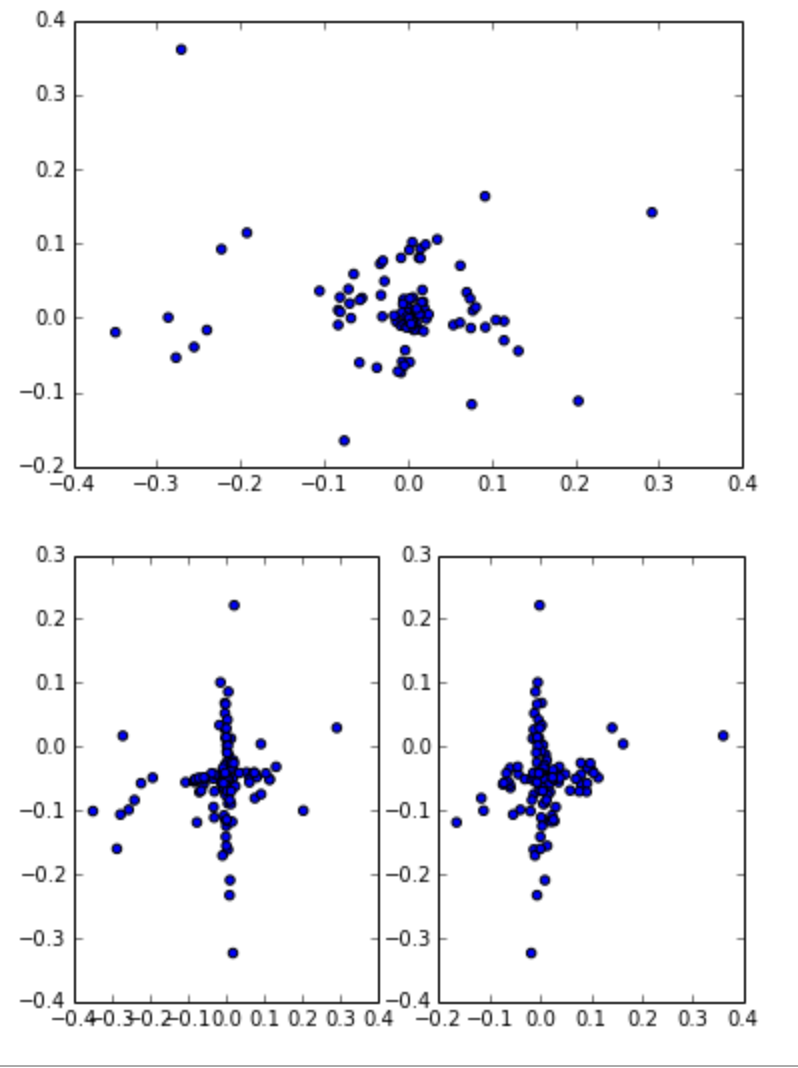
\includegraphics[width=0.45\textwidth]
  	{cluster_acc}
  \caption{Clustering of accelerometer data}
  \label{cluster}
\end{figure}

To further improve the detection of the driving mode, a low pass filter was applied to the three different acceleration signals, before performing the K-means clustering. The result for the X,Y plane is shown in figure \ref{cluster2}
\begin{figure}[h]
	\centering
	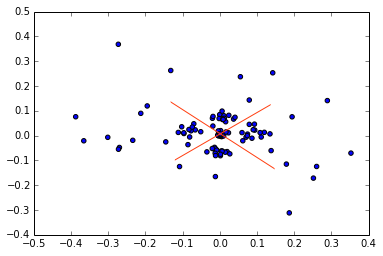
\includegraphics[width=0.45\textwidth]{cluster_acc2}
  \caption{Clustering of low-pass filtered accelerometer data}
  \label{cluster2}
\end{figure}

With the added low pass filter, a good separation between the driving modes, is apparent. the added lines indicate how to discern between the the four accelerating modes: forward, brake, left turn, and right turn. To discern between idle and cruising one have to take the Z axis signal into account as well, or consider the speed signal from the GPS.  


%\section{Future Research}\label{futurework}
In this section the planned work for the remainder of the phd study will be discussed. The focus of the section is the planned scientific contributions.

\subsection{Improving estimation of emissions for single trips}
As outlined in section \ref{Modelling}, the current modelling focus is to create and maintain national inventories, which leads to a focus on mean values for emission factors, driving patterns and trip patterns. To be able to provide personalised information on specific transportation behaviour, there is a need to provide more detailed models for the emission of single trips. In this section an outline for possible algorithms for reaching that goal is presented.

One proposal is to divide a trip into four different types of driving : Idle, accelerate, cruise and decelerate. For each type of driving a emission profile can be derived and thus the emission for each type can be determined. To total emission for a trip can then be determined as the sum of the emission for each type.

\subsubsection{Idle emissions}\label{Idle}
Detection of idle situations can be done with combination of GPS data and accelerometer data. The GPS data can be used to estimate the speed of the vehicle, and the accelerometer can be used to measure the engine speed to confirm that we are in idle mode. There are some literature about measuring emissions from idling, but it might be necessary to update with new measurements. A possible source for idle emission data could be the approval data for Danish biannual vehicle inspections, since part of the inspection is a measurement of the contents of the exhaust in idle mode.

\subsubsection{Emissions when accelerating}
The horizontal acceleration can be determined by finding the direction of gravity in respect to the device, through a variety of methods. These methods will have to be evaluated to find a suitable solution for the application at hand.
When the gravity direction has been determined, the horizontal acceleration will be either close to zero, when cruising or idle, or have a significant value due to acceleration, turning or deceleration. It is believed that it will be possible to provide a stable algorithm for detecting horizontal acceleration and distinguish between turning and acceleration.

To model the emission from an accelerating vehicle information, such as engine size and vehicle weight, is needed. This information has to be given as input to the model by the user, or be inferred from the Transportation Mode Detection part of EcoSense.

Another input to the model could be the road grade, since the engine will have to work harder, thus emitting more pollutants, if the vehicle is going uphill. By using the GPS data to get information on the position, the road grade can be gleaned from a digital road network. By fusing the information from these different sources the emission modelling  can be further improved.  

\subsubsection{Emissions when decelerating}
When decelerating, there are a couple of different situations to be ware of. The simplest situation is when the vehicle is braking using the mechanical brake. In this situation the engine will typically be in idle mode and the results from section \ref{Idle} can be reused. If the vehicle incorporate regenerative braking, motor braking or automatic transmission the situation is more complex. The proposal is to first ascertain if deceleration can be detected and then in an first approximation used the results from \ref{Idle}
\subsubsection{Emissions when cruising}
In the study of emission models, models for speed dependency of emissions have been found. These models can be used as is if we can determine that we are moving at a constant speed. These models are described in section \ref{Modelling}. The models are developed for emission modelling programs such as COPERT IV, which was developed as part of the EU project ARTEMIS. The models used in COPERT IV can be used to assign a speed dependent emission factor to specific vehicle types, engine sizes and fuel types.
 
\subsubsection{Papers}
A position paper on the state of the art of modelling emission from mobile sensing is planned.

More specialised papers detailing and evaluating the improvements made in this study is also planned.

\subsection{Correlation of trips}
In order to be able to spot inefficiencies in transportation patterns, a way of group, aggregate and correlate different trips are needed. The grouping of trips could be by persons, time of day, seasonal or geographic. The aggregation could be looking for all trips at specific location in a certain time period. Correlation is useful for finding trips which follow a certain route.

In order to solve these problems efficiently, some heuristics may be useful. If a digital road network is available for the area under consideration, each trip can be converted into a subgraph of the  digital road network, under the assumption that vehicles travels along the roads. By having the trips as a graph instead of a time series of GPS locations, will simplify the task of correlation, thus good and efficient algorithms to convert GPS traces to road network graphs is needed.
%\subsubsection{Methodology}
\subsubsection{Impact}

\subsubsection{Papers}
A paper documenting the approach and detailing the possible benefits in terms of finding opportunities for minimising the emission of pollutants through better route planning. I will attend a course at DTU Transport during the autumn concerning "Route Choice Models", to prepare for this.
\subsection{Field trials}
Among the partners in the EcoSense project are some municipalities. The interest from the municipalities in the EcoSense project are among other, to be test sites for the results coming out of the project. In return the researcher partners get real world data to learn from in future research
\subsubsection{S\o nderborg}
In the municipality of S\o nderborg, there have been a long tradition for doing projects with focus to mitigate the threat of Climate Change through minimising the emission of climate forcing gasses. The task of finding ways of minimising the emission for S\o nderborg, has been put to an organisation called "Project Zero". "Project Zero initiates and run campaigns for raising the awareness of climate gas emissions, as well as measure the effects of these campaigns. "Project Zero" has campaigns that target citizens and other campaigns that target the local industry.

As "Project Zero is a partner in EcoSense, we have the possibility to make mobile applications that underpin or are a part of the campaigns "Project Zero" runs. An interesting experiment could be measure the air pollution at the central bridge over Als-sund, and compare with the danish city canyon model OSPM, and traffic data obtained from mobile sensing.

\subsubsection{Herning}
In Herning a project called "Herning cycler til m\aa nen", Herning bikes to the moon. The goal of the project is to get the citizens of the municipality to bike the distance to the moon. To measure the distance travelled on bike, participants can download an mobile application, developed in the EcoSense project. The app sends data to the EcoSense servers, and we thus get the possibility to look into real world transportation.



\subsubsection{Papers}
It would be reasonable to document the results of this real world (or at least outside the laboratory) trials in a number of papers. Each trial has different goals but share a number of tools.

These papers would be evaluating the approach.
\subsection{Visiting researcher}
During the last 2 years of the study I plan to visit an university, to participate in the research as it is performed there. I plan to have the stay at another research group during the teaching free period in the summer of 2015. I am currently actively looking for suitable research groups in other transportation research, air pollution modelling or geographic data research.

\section{Conclusion}

In this paper we have presented a method for modelling Carbon emission from smartphone data and a method for discerning six different driving modes. The Carbon emission model is quite stable with a standard deviation of 0.02. 

The K-means based method for discerning between driving modes is able to discern between four acceleration modes (forward, brake, left turn, and right turn) and two non-accelerating modes.
\section*{Acknowledgment}
This work has been supported by The Danish Council for Strategic Research as part of the EcoSense project (11-115331).
\newpage
\pagenumbering{gobble}	
\bibliographystyle{abbrv}
\bibliography{PERCOM16}
\end{document}  












